
\section{Spray}
\label{sec:proposal}

\SPRAY is an adaptive-by-design random peer sampling protocol inspired by
\SCAMP~\cite{ganesh2001scamp,ganesh2003peer} and
\CYCLON~\cite{voulgaris2005cyclon}. It comprises three parts representing the
lifecycle of a peer in the network.  First, the joining process injects a
logarithmically growing number of arcs into the network. Hence, the number of
arcs scales with the network size.  Next, each peer runs a periodic process in
order to balance the partial views both in terms of partial view size and
uniformity of the referenced peers within them. Quickly, the overlay network
converges to a topology exposing properties close to those of random
graphs. Finally, a peer is able to leave at any time without giving notice
(equivalent to a crash) while the network properties do not degrade.

The key to adaptiveness consists in keeping a consistent global number
of arcs during the whole protocol. Indeed, unlike \CYCLON, \SPRAY is
always on the edge of the optimal number of arcs compared to the
network size. Since \SPRAY nodes never create additional arcs after
joining, any removal is a definitive loss. Thus, firstly, \SPRAY's
joining adds some arcs to the network. Secondly, \SPRAY's shuffling
preserves all arcs in the network. Thirdly, \SPRAY's leaving
cautiously removes some arcs, ideally the number of arcs introduced by
the last joining peer.

Occasionally, keeping the global number of arcs constant forces the shuffling
and the leaving processes to create \emph{duplicates} in partial views. Thus,
a partial view may contain multiple occurrences of a particular neighbor. In this
paper, we show that the number of duplicates remains low and does not
impact network connectivity.

\subsection{Joining}
\label{subsec:joining}

\SPRAY's joining algorithm is the only part of the protocol where the
global number of arcs in the network can increase. To meet the first
requirement of the problem statement, this number of arcs must grow
logarithmically compared to the network size. 
%As in \SCAMP, we assume that peers meet this constraint.
Therefore, each peer assumes that it has such a logarithmically
growing view to propagate the identity of the joining
peer. Algorithm~\ref{algo:joining} describes \SPRAY's joining
protocol. Line~\ref{line:multicast} shows that the contacted peer only
multicasts the new identity to its neighborhood. Afterwards, to limit
the risk of connection failures, each neighbor immediately adds the
joining peer to its own neighborhood. This fulfills the second
condition of the problem statement.  In total, the number of arcs in
the network increases of $1+\ln(|V^t|)$ using only
neighbor-to-neighbor interactions, which leads to a total number of
$|V^t|\ln(|V^t|)$ arcs~\cite{ganesh2001scamp}.

\begin{algorithm}[h]

\small
\SetKwProg{Function}{function}{}{}
\SetKwProg{INITIALLY}{INITIALLY}{}{}
\SetKwProg{EVENTS}{EVENTS}{}{}
\DontPrintSemicolon
\LinesNumbered

\INITIALLY {} {
  $\mathcal{P} \leftarrow \varnothing$ \Comment{the partial view is a multiset} \;
}

\EVENTS {} {
  \Function{onSubs($o$)} { % \hfill \comm{$o: origin$}
    \lFor{\textbf{each} $\langle q,\,\_\, \rangle \in\mathcal{P}$}
    {$sendTo(q,\, 'fwdSubs',\, o)$} \label{line:multicast}
  }

  \BlankLine

  \Function{onFwdSubs($o$)} {% \hfill \comm{$o: origin$}
    $\mathcal{P} \leftarrow \mathcal{P}\uplus \left\{\langle o,\, 0 \rangle\right\}$
  }

}

\caption{\label{algo:joining}The joining protocol of \SPRAY.}
\end{algorithm}

The partial view is a multiset of pairs $\langle n,\, age\rangle$
which associates each neighbor, $n$, with an age, $age$. The multiset
allows nodes to manage duplicates, while $age$ plays the same role as
in \CYCLON i.e.  it accelerates the removal of crashed/departed peers
by shuffling with the oldest neighbors first. The $onSubs$ event is
called each time a peer joins the network. $onSubs$ forwards the
identity of the joining peer to all neighbors, independently of the
age. The $onFwdSubs$ event is called when a peer receives such
forwarded subscription. It adds the peer as one of its neighbor with
an age set to $0$ meaning that it is a brand new reference.

\begin{figure*}
  \centering
  \subfloat[Figure A][$p_1$ contacts $p_2$ to join the network. $p_1$ adds
  $p_2$ to its neighborhood. $p_1$ sends its request to $p_2$.]{
    
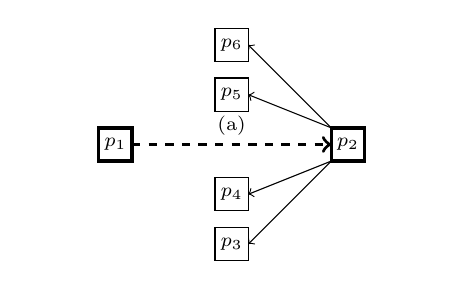
\begin{tikzpicture}[scale=1.2]

  \newcommand\X{35pt};
  \newcommand\Y{15pt};

  \draw(-0.75*\X, 0pt); %% positioning
  \draw( 2.75*\X, 0pt); %% positioning

  \scriptsize
  \draw[->,dashed,very thick](5+0*\X, 0*\Y) -- 
  node[anchor=south]{(a)}(-5+ 2*\X, 0*\Y);
  \draw[->] (-5+2*\X, 5pt) -- (5+\X, \Y);
  \draw[->] (-5+2*\X, 5pt) --  (5+\X, 2*\Y);
  \draw[->] (-5+2*\X, -5pt) -- (5+\X, -\Y);
  \draw[->] (-5+2*\X, -5pt) -- (5+\X, -2*\Y);

  \draw[fill=white, very thick]
  (0*\X, 0*\Y) node{$p_1$} +(-5pt,-5pt) rectangle +(5pt,5pt);
  \draw[fill=white, very thick]
  (2*\X, 0*\Y) node{$p_2$} +(-5pt,-5pt) rectangle +(5pt,5pt);

  \draw[fill=white](1*\X,2*\Y) node{$p_6$} +(-5pt,-5pt) rectangle +(5pt,5pt);
  \draw[fill=white](1*\X,1*\Y) node{$p_5$} +(-5pt,-5pt) rectangle +(5pt,5pt);
  \draw[fill=white](1*\X,-1*\Y) node{$p_4$} +(-5pt,-5pt) rectangle +(5pt,5pt);
  \draw[fill=white](1*\X,-2*\Y) node{$p_3$} +(-5pt,-5pt) rectangle +(5pt,5pt);
  
\end{tikzpicture}}
  \hspace{8pt}
  \subfloat[Figure B][The $onSubs(p_1)$ event is raised at $p_2$
  which forwards the subscription to its neighbors.]{
    
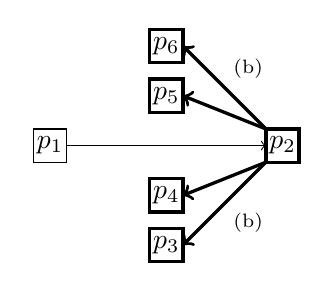
\begin{tikzpicture}[scale=1.2]

  \newcommand\X{35pt};
  \newcommand\Y{15pt};

  \scriptsize
  \draw[->](5+0*\X, 0*\Y) -- (-5+ 2*\X, 0*\Y);
  \draw[->, very thick] (-5+2*\X, 5pt) -- (5+\X, \Y);
  \draw[->, very thick] (-5+2*\X, 5pt) --
  node[anchor=south west]{(b)} (5+\X, 2*\Y);
  \draw[->, very thick] (-5+2*\X, -5pt) -- (5+\X, -\Y);
  \draw[->, very thick] (-5+2*\X, -5pt) --
  node[anchor=north west]{(b)}(5+\X, -2*\Y);

  \normalsize
  \draw[fill=white]
  (0*\X, 0*\Y) node{$p_1$} +(-5pt,-5pt) rectangle +(5pt,5pt);
  \draw[fill=white, very thick]
  (2*\X, 0*\Y) node{$p_2$} +(-5pt,-5pt) rectangle +(5pt,5pt);

  \draw[fill=white, very thick]
  (1*\X,2*\Y) node{$p_6$} +(-5pt,-5pt) rectangle +(5pt,5pt);
  \draw[fill=white, very thick]
  (1*\X,1*\Y) node{$p_5$} +(-5pt,-5pt) rectangle +(5pt,5pt);
  \draw[fill=white, very thick]
  (1*\X,-1*\Y) node{$p_4$} +(-5pt,-5pt) rectangle +(5pt,5pt);
  \draw[fill=white, very thick]
  (1*\X,-2*\Y) node{$p_3$} +(-5pt,-5pt) rectangle +(5pt,5pt);

\end{tikzpicture}}
  \hspace{8pt}
  \subfloat[Figure C][The $onFwdSubs(p_1)$ event is raised at $p_{3-6}$. The 
  peers add $p_1$ to their neighborhood.]{
    
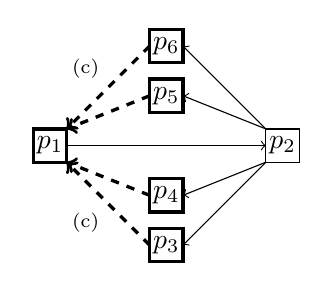
\begin{tikzpicture}[scale=1.2]

  \newcommand\X{35pt};
  \newcommand\Y{15pt};

  \scriptsize
  \draw[->](5+0*\X, 0*\Y) -- (-5+ 2*\X, 0*\Y);
  \draw[->] (-5+2*\X, 5pt) -- (5+\X, \Y);
  \draw[->] (-5+2*\X, 5pt) -- (5+\X, 2*\Y);
  \draw[->] (-5+2*\X, -5pt) -- (5+\X, -\Y);
  \draw[->] (-5+2*\X, -5pt) -- (5+\X, -2*\Y);

  \draw[->,dashed, very thick](-5+\X, 2*\Y) --
  node[anchor=south east]{(c)} ( 5pt,5pt);
  \draw[->,dashed, very thick](-5+\X, 1*\Y) -- ( 5pt,5pt);
  \draw[->,dashed, very thick](-5+\X, -1*\Y) -- ( 5pt,-5pt);
  \draw[->,dashed, very thick](-5+\X, -2*\Y) --
  node[anchor=north east]{(c)}( 5pt,-5pt);

  \normalsize
  \draw[fill=white, very thick]
  (0*\X, 0*\Y) node{$p_1$} +(-5pt,-5pt) rectangle +(5pt,5pt);
  \draw[fill=white]
  (2*\X, 0*\Y) node{$p_2$} +(-5pt,-5pt) rectangle +(5pt,5pt);

  \draw[fill=white, very thick]
  (1*\X,2*\Y) node{$p_6$} +(-5pt,-5pt) rectangle +(5pt,5pt);
  \draw[fill=white, very thick]
  (1*\X,1*\Y) node{$p_5$} +(-5pt,-5pt) rectangle +(5pt,5pt);
  \draw[fill=white, very thick]
  (1*\X,-1*\Y) node{$p_4$} +(-5pt,-5pt) rectangle +(5pt,5pt);
  \draw[fill=white, very thick]
  (1*\X,-2*\Y) node{$p_3$} +(-5pt,-5pt) rectangle +(5pt,5pt);
 

\end{tikzpicture}}
  \caption{\label{fig:joiningexample}Example of the \SPRAY's joining
    protocol.}
\end{figure*}

Figure~\ref{fig:joiningexample} depicts a joining scenario.  Peer
$p_1$ contacts $p_2$ to join the network composed of $\{p_2$, $p_3$,
$p_4$, $p_5$, $p_6\}$. For simplicity, the figure shows only the new
arcs and the neighborhoods of $p_1$ and $p_2$. Peer $p_1$ directly adds
$p_2$ in its partial view. Peer $p_2$ forwards the identity of $p_1$
to its neighborhood. Each of these neighbors adds $p_1$ in their
partial view. In total, \SPRAY establishes 5 connections and the
network is connected.

Unfortunately, the partial views of the newest peers are clearly unbalanced and
violate the first condition of our problem statement. The periodic protocol
described in the next section will re-balance the partial views.

\subsection{Shuffling}
\label{subsec:cyclic}

Unlike \CYCLON, \SPRAY shuffles partial views of different sizes. The
shuffling balances the partial view sizes and randomly mixes the
neighborhoods between peers. Nevertheless, the global number of arcs
in the network remains unchanged.

In \SPRAY's shuffling protocol, each of the involved peers sends half of its
partial view to the other. After integration, their view sizes both tend to the
average of their initial sizes. The sum of their elements remains unchanged. In
order to keep the arc number invariant, the partial views of \SPRAY are
multisets. If a peer receives an already known reference, it still stores it,
yet as a duplicate. Thus, the \SPRAY's shuffling protocol never increases nor
decreases the arc count.

If duplicates have a negative impact on network properties, most of
them disappear after shuffling and they proportionally become
negligible as the network grows.

\begin{algorithm}[h]
  
\small
\algrenewcommand{\algorithmiccomment}[1]{\hskip2em$\rhd$ #1}

\newcommand{\comm}[1]{$\rhd$ #1}

\algblockdefx[act]{act}{endAct}
  [0] {\textbf{ACTIVE THREAD:}}

\algsetblockdefx[pas]{pas}{endPas}
{65535}{}
[0] {\textbf{PASSIVE THREAD:}}


\newcommand{\LINEFOR}[2]{%
  \algorithmicfor\ {#1}\ \algorithmicdo\ {#2} %
  }

\newcommand{\LINEIFTHEN}[2]{%
  \algorithmicif\ {#1}\ \algorithmicthen\ {#2} %
  }

\newcommand{\INDSTATE}[1][1]{\State\hspace{\algorithmicindent}}

\begin{algorithmic}[1]
  \Statex
  \act
    \Function{loop}{ } \hfill \comm{Every $\Delta\,t$}
    \State $\mathcal{P} \leftarrow incrementAge(\mathcal{P})$;
    \State \textbf{let} $ \langle q,\, age \rangle \leftarrow getOldest(\mathcal{P})$;
    \State \textbf{let} $sample \leftarrow $ \label{line:samplesize}
    \Statex \hfill $getSample(\mathcal{P}\setminus\left\{\langle q, age\rangle\right\}, \left \lceil{|\mathcal{P}|\over{2}} \right \rceil-1) \uplus \left\{\langle p, 0 \rangle\right\}$;
    \State $sample \leftarrow replace(sample,\,q,\,p)$; \label{line:replace1}
    \State $sendTo(q,\, 'exchange',\, sample)$;
    \State \textbf{let} $sample'\leftarrow receiveFrom(q)$;
    \State $sample \leftarrow replace(sample,\,p,\,q)$;
    \State $\mathcal{P} \leftarrow (\mathcal{P} \setminus sample) \uplus
    sample'$;
    \EndFunction
  \endAct
  
  \pas
    \Function{onExchange}{$o,\, sample$} \hfill \comm{$o: origin$}
    \State \textbf{let} $sample' \leftarrow getSample(\mathcal{P} ,\, \left\lceil |\mathcal{P}|\over{2} \right\rceil )$;
    \State $sample' \leftarrow replace(sample',\,o,\,p);$ \label{line:replace2}
    \State $sendTo(o ,\, sample')$;
    \State $sample' \leftarrow replace(sample',\,p,\,o)$;
    \State $\mathcal{P} \leftarrow (\mathcal{P} \setminus sample') \uplus
    sample$; 
    \EndFunction
%%  \endPas
  
\end{algorithmic}

  \caption{\label{algo:scamplon}The cyclic protocol of \SPRAY.}
\end{algorithm}

Algorithm~\ref{algo:scamplon} shows the \SPRAY protocol running at
each peer. It is divided between an active thread looping to update
the partial view, and a passive thread which reacts to messages. The
functions which are not explicitly defined are the following:
\begin{compactitem}
\item \textsc{incrementAge}$(view)$: increments the age of each element in the view
  and returns the modified view.
\item \textsc{getOldest}$(view)$: retrieves the oldest peer contained in the view.
\item \textsc{getSample}$(view, \, size)$: returns a sample of the view containing
  $size$ elements.
\item \textsc{replace}$(view,\,old,\,new)$: replaces all the occurrences of the
  $old$ element in the view by the $new$ element and returns the
  modified view.
\item \textsc{rand}$()$: generates a random floating-point number between $0$
  and $1$.
\end{compactitem}

In the active thread, Function \textsc{loop} is called every $\Delta t$ time
units. First, the function increments the age of each neighbor in
$\mathcal{P}$. Then, it chooses the oldest peer $q$ to exchange a
subset of its partial view. If Peer $q$ cannot be reached (i.e. it
crashed/left), peer $p$ executes the crash-handling function
(see Section~\ref{subsec:leaving}) and repeats the process until it
finds a reachable peer $q$. Thus, the aging process (which is an
inheritance from \CYCLON) speeds up the removal of crashed or departed
peers. Once it finds a reachable neighbor $q$, Peer $p$ selects a
sample of its partial view, excluding one occurrence of $q$ and
including itself. The size of this sample is half of its partial view,
with at least one peer: the initiating peer
(see Line~\ref{line:samplesize}). The answer of $q$ contains half of
its partial view. Since peers can appear multiple times in
$\mathcal{P}$, the exchanging peers may send references to the other
peer, e.g., Peer $p$'s sample can contain references to $q$. Such
sample, without further processing, would create self-loop ($q$'s
partial view contains references to $q$). To alleviate this
undesirable behavior, all occurrences of the other peer are replaced
with the emitting peer
(see Line~\ref{line:replace1},~\ref{line:replace2}).  Afterwards, both
of them remove the sample they sent from their view and add the
received sample.

\begin{figure*}
  \centering
  \subfloat[Figure A]
  [Peer $p_6$ initiates the exchange with $p_1$ by sending to the
  latter the multiset $\{p_6,\,p_9\}$.]{
    
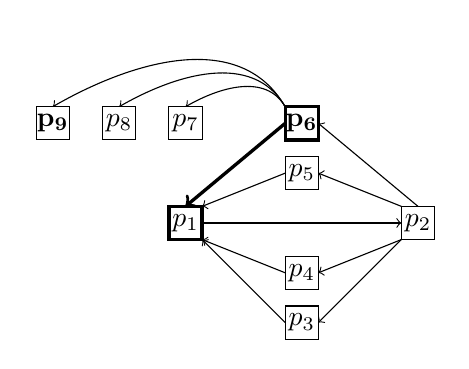
\begin{tikzpicture}[scale=1.2]

  \newcommand\X{35pt};
  \newcommand\Y{15pt};

  \draw[->](5+0*\X, 0*\Y) -- (-5+ 2*\X, 0*\Y); %% 1 -> 2
  \draw[->] (-5+2*\X, 5pt) -- (5+\X, \Y);
  \draw[->](2*\X,5pt) -- (5+1*\X, 2*\Y); %% 2 -> 6
  \draw[->] (-5+2*\X, -5pt) -- (5+\X, -\Y);
  \draw[->] (-5+2*\X, -5pt) -- (5+\X, -2*\Y);

  \draw[->,very thick](-5+\X,2*\Y) -- (0pt,5pt); %% 6 -> 1

  \draw[->](-5+\X, 1*\Y) -- ( 5pt,5pt);
  \draw[->](-5+\X, -1*\Y) -- ( 5pt,-5pt);
  \draw[->](-5+\X, -2*\Y) -- ( 5pt,-5pt);

  \draw[->](-5+\X, 5+2*\Y)to[out=120,in=30](0pt,5+2*\Y); %% 6 -> 7
  \draw[->](-5+\X, 5+2*\Y)to[out=120,in=30](-5-\Y ,5+2*\Y); %% 6 -> 8
  \draw[->](-5+\X, 5+2*\Y)to[out=120,in=30](-10-2*\Y,5+2*\Y); %% 6 -> 9

  \normalsize
  \draw[fill=white, very thick]
  (0*\X, 0*\Y) node{$p_1$} +(-5pt,-5pt) rectangle +(5pt,5pt);
  \draw[fill=white](2*\X, 0*\Y) node{$p_2$} +(-5pt,-5pt) rectangle +(5pt,5pt);

  \draw[fill=white,very thick]
  (1*\X,2*\Y) node{$\mathbf{p_6}$} +(-5pt,-5pt) rectangle +(5pt,5pt);
  \draw[fill=white](1*\X,1*\Y) node{$p_5$} +(-5pt,-5pt) rectangle +(5pt,5pt);
  \draw[fill=white](1*\X,-1*\Y) node{$p_4$} +(-5pt,-5pt) rectangle +(5pt,5pt);
  \draw[fill=white](1*\X,-2*\Y) node{$p_3$} +(-5pt,-5pt) rectangle +(5pt,5pt);

  \draw[fill=white]( 0*\X,2*\Y)
  node{$p_7$} +(-5pt,-5pt) rectangle +(5pt,5pt);
  \draw[fill=white](-5+-\Y,2*\Y)node{$p_8$} +(-5pt,-5pt) rectangle +(5pt,5pt);
  \draw[fill=white](-10+-2*\Y,2*\Y) node{$\mathbf{p_9}$} +(-5pt,-5pt) rectangle +(5pt,5pt);
  

\end{tikzpicture}}
  \hspace{10pt}
  \subfloat[Figure B][Peer $p_1$ receives $p_6$'s message. 
  It sends back the multiset $\{p_2\}$ and adds $\{p_6,\,p_9\}$ to its 
  partial view.]{
    
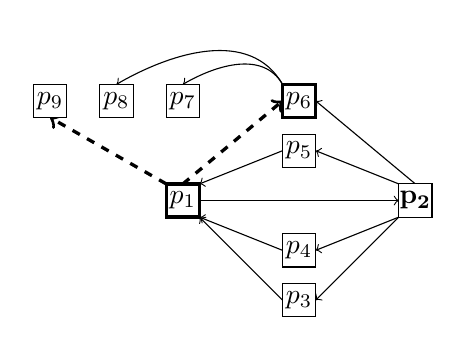
\begin{tikzpicture}[scale=1.2]

  \newcommand\X{35pt};
  \newcommand\Y{15pt};

  \draw[->](5+0*\X, 0*\Y) -- (-5+ 2*\X, 0*\Y); %% 1 -> 2
  \draw[->] (-5+2*\X, 5pt) -- (5+\X, \Y);
  \draw[->](2*\X,5pt) -- (5+1*\X, 2*\Y); %% 2 -> 6
  \draw[->] (-5+2*\X, -5pt) -- (5+\X, -\Y);
  \draw[->] (-5+2*\X, -5pt) -- (5+\X, -2*\Y);

  \draw[->,dashed, very thick](0pt,5pt)--(-5+\X, 2*\Y); %% 1 -> 6

  \draw[->](-5+\X, 1*\Y) -- ( 5pt,5pt);
  \draw[->](-5+\X, -1*\Y) -- ( 5pt,-5pt);
  \draw[->](-5+\X, -2*\Y) -- ( 5pt,-5pt);

  \draw[->](-5+\X, 5+2*\Y)to[out=120,in=30](0pt,5+2*\Y); %% 6 -> 7
  \draw[->](-5+\X, 5+2*\Y)to[out=120,in=30](-5-\Y ,5+2*\Y); %% 6 -> 8
  
  \draw[->,dashed, very thick](-5pt,5pt)--(-10-2*\Y,-5+2*\Y); %% 1 -> 9

  \normalsize
  \draw[fill=white, very thick]
  (0*\X, 0*\Y) node{$p_1$} +(-5pt,-5pt) rectangle +(5pt,5pt);
  \draw[fill=white](2*\X, 0*\Y)
  node{$\mathbf{p_2}$} +(-5pt,-5pt) rectangle +(5pt,5pt);

  \draw[fill=white,very thick]
  (1*\X,2*\Y) node{$p_6$} +(-5pt,-5pt) rectangle +(5pt,5pt);
  \draw[fill=white](1*\X,1*\Y) node{$p_5$} +(-5pt,-5pt) rectangle +(5pt,5pt);
  \draw[fill=white](1*\X,-1*\Y) node{$p_4$} +(-5pt,-5pt) rectangle +(5pt,5pt);
  \draw[fill=white](1*\X,-2*\Y) node{$p_3$} +(-5pt,-5pt) rectangle +(5pt,5pt);

  \draw[fill=white]( 0*\X,2*\Y)
  node{$p_7$} +(-5pt,-5pt) rectangle +(5pt,5pt);
  \draw[fill=white](-5+-\Y,2*\Y)node{$p_8$} +(-5pt,-5pt) rectangle +(5pt,5pt);
  \draw[fill=white](-10+-2*\Y,2*\Y) node{$p_9$} +(-5pt,-5pt) rectangle +(5pt,5pt);
  

\end{tikzpicture}}
  \hspace{10pt}
  \subfloat[Figure C][Peer $p_6$ receives $p_1$'s response, it
  adds $\{p_2\}$ to its partial view.]{
    
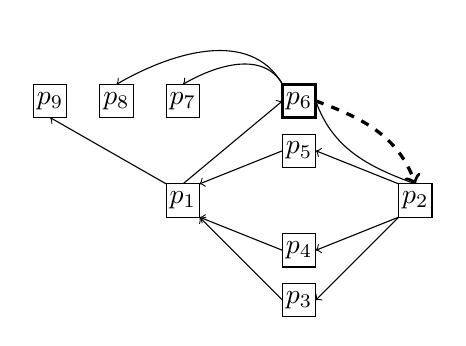
\begin{tikzpicture}[scale=1.2]

  \newcommand\X{35pt};
  \newcommand\Y{15pt};

  \draw[->] (-5+2*\X, 5pt) -- (5+\X, \Y);
  \draw[->,dashed, very thick]
  (5+\X, 2*\Y)to[out=-20,in=110](2*\X, 5pt); %% 6 -> 2
  \draw[->](2*\X,5pt)to[out=160,in=-70](5+1*\X, 2*\Y); %% 2 -> 6
  \draw[->] (-5+2*\X, -5pt) -- (5+\X, -\Y);
  \draw[->] (-5+2*\X, -5pt) -- (5+\X, -2*\Y);

  \draw[->](0pt,5pt)--(-5+\X, 2*\Y); %% 1 -> 6

  \draw[->](-5+\X, 1*\Y) -- ( 5pt,5pt);
  \draw[->](-5+\X, -1*\Y) -- ( 5pt,-5pt);
  \draw[->](-5+\X, -2*\Y) -- ( 5pt,-5pt);

  \draw[->](-5+\X, 5+2*\Y)to[out=120,in=30](0pt,5+2*\Y); %% 6 -> 7
  \draw[->](-5+\X, 5+2*\Y)to[out=120,in=30](-5-\Y ,5+2*\Y); %% 6 -> 8
  
  \draw[->](-5pt,5pt)--(-10-2*\Y,-5+2*\Y); %% 1 -> 9

  \normalsize
  \draw[fill=white]
  (0*\X, 0*\Y) node{$p_1$} +(-5pt,-5pt) rectangle +(5pt,5pt);
  \draw[fill=white](2*\X, 0*\Y) node{$p_2$} +(-5pt,-5pt) rectangle +(5pt,5pt);

  \draw[fill=white,very thick]
  (1*\X,2*\Y) node{$p_6$} +(-5pt,-5pt) rectangle +(5pt,5pt);
  \draw[fill=white](1*\X,1*\Y) node{$p_5$} +(-5pt,-5pt) rectangle +(5pt,5pt);
  \draw[fill=white](1*\X,-1*\Y) node{$p_4$} +(-5pt,-5pt) rectangle +(5pt,5pt);
  \draw[fill=white](1*\X,-2*\Y) node{$p_3$} +(-5pt,-5pt) rectangle +(5pt,5pt);

  \draw[fill=white]( 0*\X,2*\Y)
  node{$p_7$} +(-5pt,-5pt) rectangle +(5pt,5pt);
  \draw[fill=white](-5+-\Y,2*\Y)node{$p_8$} +(-5pt,-5pt) rectangle +(5pt,5pt);
  \draw[fill=white](-10+-2*\Y,2*\Y) node{$p_9$} +(-5pt,-5pt) rectangle +(5pt,5pt);
  

\end{tikzpicture}}
  \caption{\label{fig:cyclicexample}Example of the \SPRAY's shuffling
    protocol. }
\end{figure*}

Figure~\ref{fig:cyclicexample} depicts \SPRAY's shuffling procedure. This
scenario follows from Figure~\ref{fig:joiningexample}: Peer $p_1$ just joined
the network. Peer $p_6$ initiates an exchange with $p_1$ (the oldest among 
$p_6$'s partial view). It randomly chooses
$\left\lceil{|\mathcal{P}_6|\div 2} - 1 \right \rceil = 1$ peer among its
neighborhood. In this case, it picks $p_9$ from $\{p_7,\,p_8,\,p_9\}$.  It sends
the chosen peer plus its own identity to Peer $p_1$. In response, the latter
picks $\left\lceil{|\mathcal{P}_1|\div 2}\right\rceil = 1$ peer from its partial
view. It sends back its sole neighbor $p_2$ and directly adds the received
neighbor to its partial view. After receipt, Peer $p_6$ removes the sent
neighbor from its partial view, removes an occurrence of $p_1$, and adds the
received peer from $p_1$. Peers $\{p_6,\,p_9\}$ compose $p_1$'s partial
view. Peers $\{p_2,\,p_7,\,p_8\}$ compose that of $p_6$.

The example shows that, at first, the initiating peer has $4$ peers in
its partial view, while the receiving peer has only $1$ peer.
After the exchange, the former has $3$ neighbors including $1$ new
peer. The receiving peer has $2$ neighbors, and both of them are
new. Thus, the periodic procedure tends to even out the partial view
sizes of network members. It also scatters neighbors in order to remove
the highly clustered groups which may appear because of the joining
protocol.

Concerning the convergence time of the shuffling algorithm, there
exists a close relationship between \SPRAY and the proactive
aggregation protocol introduced
in~\cite{jelasity2004epidemic}. Given a
distribution of values associated with peers, and under the assumption
of a sufficiently random peer sampling, such an aggregation protocol
yields the following mean $\mu$, and variance $\sigma^2$, at cycle
$i$;
\begin{center}
  $\mu_i = {1\over{|V^t|}} \sum\limits_{x \in V^t} a_{i,\,x}$
  \hfill
  $\sigma^2_i = {1\over{|V^t|-1}}\sum\limits_{x \in V^t}
  (a_{i,\,x} - \mu_i)^2$
\end{center}
where $a_{i,\,x}$ is the value held by Peer $p_x$ at cycle $i$. The
estimated variance must converge to $0$ over cycles. In other terms,
the values tend to be the same over cycles. In the \SPRAY case, the
value $a_{i,\,x}$ is the partial view size of Peer $p_x$ at cycle
$i$. Indeed, each exchange from Peer $p_1$ to Peer $p_2$ is an
aggregation resulting to:
$|\mathcal{P}_1|\approx|\mathcal{P}_2|\approx{(|\mathcal{P}_1| +
  |\mathcal{P}_2|) \div 2}$.  Furthermore, at each cycle, each peer is
involved in the exchange protocol at least once (they initiate one),
and in the best case $1+Poisson(1)$ (they initiate one and, on average,
each peer receives another one). This relation being established, we
know that \SPRAY's partial view sizes converge exponentially fast to
the global average size. Additionally, we know that each cycle
decreases their variance in the overall system at a rate comprised
between ${1\div 2}$ and $1\div ({2\sqrt{\text{e}}})$.

The shuffling algorithm provides adaptiveness at the cost of
duplicates. Averaging the partial view sizes over exchanges quickly
converges to a network topology where the partial views are balanced.

\subsection{Leaving or crashing}
\label{subsec:leaving}

In \SPRAY, peers can leave the network without notice. We make no
distinction between node departures and crashes, but the protocol must
react to both of them. Without such a reaction, the network could
collapse due to an over zealous removal of arcs. When a peer joins the
network, it injects $1+\ln(|V^t|)$ arcs. Nevertheless, after few
exchanges, the partial view of the joining peer becomes populated with
more neighbors. Then, if this peer leaves, it removes $\ln(|V^t|)$
arcs from its partial view, and another $\ln(|V^t|)$ arcs from peers
which have this peer in their partial views. Therefore, without any
crash handler, we remove $2\ln(|V^t|)$ connections instead of
$1+\ln(|V^t|)$. To alleviate this issue, each peer that detects a
crash may reestablish a connection with anyone in its neighborhood
(which will spread in the network over the exchanges). The probability
of reestablishing a connection is $1-{1\div{|\mathcal{P}|}}$. Since
${|\mathcal{P}|}\approx \ln(|V^t|)$ peers have the crashed peer in
their partial view, it is likely that all of them will reestablish a
connection, except one. Therefore, when a peer leaves, it
approximately removes the number of connections injected by the most
recently joined node.

\begin{algorithm}[h]
  
\small
\SetKwProg{Function}{function}{}{}
\SetKwComment{tcp}{$\triangleright$~}{}
\DontPrintSemicolon
\LinesNumbered

\newcommand{\LET}[0]{\textbf{let}\xspace}
\newcommand{\FROM}[0]{\textup{\textbf{from}}\xspace}
\newcommand{\TO}[0]{\textup{\textbf{to}}\xspace}

\Function{\textup{onPeerDown ($q$)} \tcp*[f]{$q$: crashed/departed}} {
  \LET $occ \leftarrow 0$ \;

  \ForEach(\tcp*[f]{remove and count}) { $\langle n, age\rangle \in \mathcal{P}$ }  {
    \If {$n=q$} {
       $\mathcal{P} \leftarrow \mathcal{P}\setminus \{\langle n,\,age\rangle \}$ \;
       $occ \leftarrow occ + 1$ \;
    }
  }

  \For{$i$ \FROM $0$ \TO $occ$} {
    \tcp*[l]{probabilistically duplicates}

    \If{$\textup{rand( )}>{1\div{(|\mathcal{P}|+occ}})$} {
       \LET $\langle n,\,\_ \,\rangle \leftarrow
         \mathcal{P}[\left\lfloor \textup{rand( )}*|\mathcal{P}|\right\rfloor]$ \;
       $\mathcal{P} \leftarrow \mathcal{P} \uplus \left\{\langle n,\, 0\rangle\right\}$
    }
  }
}

\BlankLine

\Function{\textup{onArcDown($q$, $age$)} \tcp*[f]{$q$: arc arrival}} {
  $\mathcal{P} \leftarrow \mathcal{P}\setminus \{\langle q, age\rangle \}$ \;
  \tcp*[l]{systematically duplicates}
  \LET $\langle n, \_ \rangle \leftarrow
  \mathcal{P}[\left\lfloor \textup{rand( )}*|\mathcal{P}|\right\rfloor]$ \;
  $\mathcal{P} \leftarrow \mathcal{P} \uplus \left\{\langle n, 0\rangle\right\}$ \;

}

  \caption{\label{algo:unreachable}The crash/departure handler of \SPRAY.}
\end{algorithm}

Algorithm~\ref{algo:unreachable} shows the manner in which \SPRAY deals with
departures and crashes.  Function \textsc{onPeerDown} shows the reaction of \SPRAY
when peer $q$ is detected as crashed or departed. A first loop counts the
occurrences of this neighbor in the partial view, and removes all of
them. Then, the second loop probabilistically duplicates the reference of 
known peers. The probability depends on the partial view size before the
removals.

Figure~\ref{fig:crashexample} depicts \SPRAY's crash/leaving handler. The
scenario follows from prior examples after few other exchanges. Peer $p_1$
leaves the network without giving notice. With it, $7$ connections are
down. Peers $p_3$, $p_4$, and $p_5$ have the crashed/left peer in their partial
view. Peer $p_5$ has $1-{1\div{|\mathcal{P}_5|}}={2\div{3}}$ chance to replace
the dead connections. In this case, it duplicates the connection to
$p_{13}$. Identically, $p_3$ and $p_4$ detect the crash/leaving and run the
appropriate operation. Only $p_3$ duplicates one of its connections. In total,
$5$ connections have been removed.


%% figure related to crash/departure, here to be on top of page
\begin{figure*}
  \centering
  \subfloat[Figure A][Peer $p_1$ crashes. A lot of connections are down.]{
    
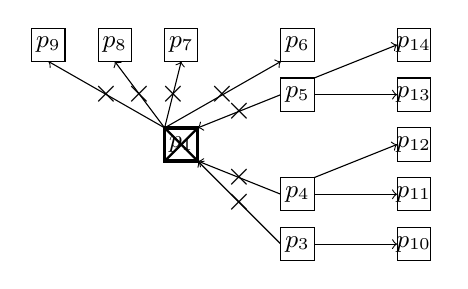
\begin{tikzpicture}[scale=1.2]

  \newcommand\X{35pt};
  \newcommand\Y{15pt};
  \large
  \draw[->](-5+\X, 1*\Y) --node{$\times$} ( 5pt,5pt);
  \draw[->](-5+\X, -1*\Y) --node{$\times$} ( 5pt,-5pt);
  \draw[->](-5+\X, -2*\Y) --node{$\times$} ( 5pt,-5pt);

  \draw[->](-5pt,5pt)--node{$\times$}(-10-2*\Y,-5+2*\Y); %% 1 -> 9
  \draw[->](-5pt,5pt)--node{$\times$}(-5-1*\Y,-5+2*\Y); %% 1 ->8 
  \draw[->](-5pt,5pt)--node{$\times$}(0pt,-5+2*\Y); %% 1 -> 7
  \draw[->](-5pt,5pt)--node{$\times$}(-5+\X,-5+2*\Y); %% 1 -> 6
  \normalsize
  \draw[->](5+ 1*\X, 5+ 1*\Y)--(-5+2*\X, 2*\Y); %% 5 -> 14
  \draw[->](5+1*\X,  1*\Y)--(-5+2*\X, 1*\Y); %% 5 -> 13 
  
  \draw[->](5+\X, 5-\Y) -- (-5+2*\X,0pt); %% 4 -> 12
  \draw[->](5+\X, -\Y) -- (-5+2*\X, -\Y); %% 4 -> 11
  
  \draw[->](5+\X, -2*\Y) -- (-5+2*\X, -2*\Y);
  
  \small
  \draw[fill=white,very thick]
  (0*\X, 0*\Y) node{$p_1$} +(-5pt,-5pt) rectangle +(5pt,5pt);
  \draw[thick] (-5pt,-5pt) -- (5pt,5pt);
  \draw[thick] (-5pt, 5pt) -- (5pt,-5pt);
  
  \draw[fill=white]
  (1*\X,1*\Y) node{$p_5$} +(-5pt,-5pt) rectangle +(5pt,5pt);
  \draw[fill=white]
  (1*\X,-1*\Y) node{$p_4$} +(-5pt,-5pt) rectangle +(5pt,5pt);
  \draw[fill=white]
  (1*\X,-2*\Y) node{$p_3$} +(-5pt,-5pt) rectangle +(5pt,5pt);

  \draw[fill=white](\X,2*\Y) node{$p_6$} +(-5pt,-5pt) rectangle +(5pt,5pt);

  \draw[fill=white]( 0*\X,2*\Y)
  node{$p_7$} +(-5pt,-5pt) rectangle +(5pt,5pt);
  \draw[fill=white](-5+-\Y,2*\Y)node{$p_8$} +(-5pt,-5pt) rectangle +(5pt,5pt);
  \draw[fill=white](-10+-2*\Y,2*\Y) node{$p_9$} +(-5pt,-5pt) rectangle +(5pt,5pt);
  
  \draw[fill=white](2*\X,2*\Y)node{$p_{14}$} +(-5pt,-5pt) rectangle +(5pt,5pt);
  \draw[fill=white](2*\X,1*\Y)node{$p_{13}$} +(-5pt,-5pt) rectangle +(5pt,5pt);
  \draw[fill=white](2*\X,0*\Y)node{$p_{12}$} +(-5pt,-5pt) rectangle +(5pt,5pt);
  \draw[fill=white](2*\X,-1*\Y)node{$p_{11}$}+(-5pt,-5pt) rectangle +(5pt,5pt);
  \draw[fill=white](2*\X,-2*\Y)node{$p_{10}$}+(-5pt,-5pt) rectangle +(5pt,5pt);

\end{tikzpicture}}
  \hspace{10pt}
  \subfloat[Figure B][The peers $p_{3-5}$ notice that they cannot 
  reach $p_1$ anymore.]{
    
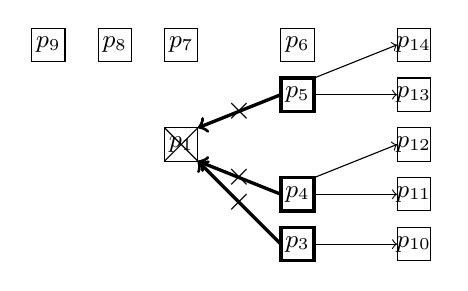
\begin{tikzpicture}[scale=1.2]

  \newcommand\X{35pt};
  \newcommand\Y{15pt};

  \large
  \draw[->, very thick](-5+\X, 1*\Y) -- node{$\times$} ( 5pt,5pt);
  \draw[->, very thick](-5+\X, -1*\Y) --node{$\times$} ( 5pt,-5pt);
  \draw[->, very thick](-5+\X, -2*\Y) --node{$\times$} ( 5pt,-5pt);

  \normalsize

  \draw[->](5+ 1*\X, 5+ 1*\Y)--(-5+2*\X, 2*\Y); %% 5 -> 14
  \draw[->](  5+1*\X, 1*\Y)--(-5+2*\X, 1*\Y); %% 5 -> 13 (v)
  
  \draw[->](5+\X, 5-\Y) -- (-5+2*\X,0pt); %% 4 -> 12
  \draw[->](5+\X, -\Y) -- (-5+2*\X, -\Y); %% 4 -> 11
  
  \draw[->](5+\X, -2*\Y) -- (-5+2*\X, -2*\Y);
  
  \small
  \draw[fill=white]
  (0*\X, 0*\Y) node{$p_1$} +(-5pt,-5pt) rectangle +(5pt,5pt);
  \draw (-5pt,-5pt) -- (5pt,5pt);
  \draw (-5pt, 5pt) -- (5pt,-5pt);
  
  \draw[fill=white, very thick]
  (1*\X,1*\Y) node{$p_5$} +(-5pt,-5pt) rectangle +(5pt,5pt);
  \draw[fill=white, very thick]
  (1*\X,-1*\Y) node{$p_4$} +(-5pt,-5pt) rectangle +(5pt,5pt);
  \draw[fill=white, very thick]
  (1*\X,-2*\Y) node{$p_3$} +(-5pt,-5pt) rectangle +(5pt,5pt);

  \draw[fill=white](\X,2*\Y) node{$p_6$} +(-5pt,-5pt) rectangle +(5pt,5pt);

  \draw[fill=white]( 0*\X,2*\Y)
  node{$p_7$} +(-5pt,-5pt) rectangle +(5pt,5pt);
  \draw[fill=white](-5+-\Y,2*\Y)node{$p_8$} +(-5pt,-5pt) rectangle +(5pt,5pt);
  \draw[fill=white](-10+-2*\Y,2*\Y) node{$p_9$} +(-5pt,-5pt) rectangle +(5pt,5pt);
  
  \draw[fill=white](2*\X,2*\Y)node{$p_{14}$} +(-5pt,-5pt) rectangle +(5pt,5pt);
  \draw[fill=white](2*\X,1*\Y)node{$p_{13}$} +(-5pt,-5pt) rectangle +(5pt,5pt);
  \draw[fill=white](2*\X,0*\Y)node{$p_{12}$} +(-5pt,-5pt) rectangle +(5pt,5pt);
  \draw[fill=white](2*\X,-1*\Y)node{$p_{11}$}+(-5pt,-5pt) rectangle +(5pt,5pt);
  \draw[fill=white](2*\X,-2*\Y)node{$p_{10}$}+(-5pt,-5pt) rectangle +(5pt,5pt);

\end{tikzpicture}}
  \hspace{10pt}
  \subfloat[Figure C][The peers $p_3$ and $p_5$ create
  a duplicate of one of their existing neighbor.]{
    
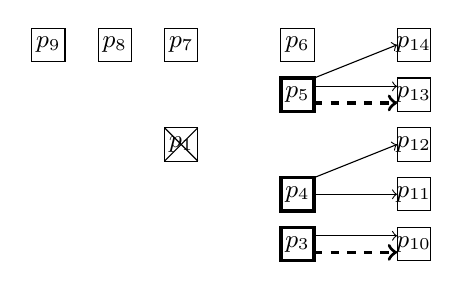
\begin{tikzpicture}[scale=1.2]

  \newcommand\X{35pt};
  \newcommand\Y{15pt};

  \draw[->](5+ 1*\X, 5+ 1*\Y)--(-5+2*\X, 2*\Y); %% 5 -> 14
  \draw[->](5+1*\X, 2.5+ 1*\Y)--(-5+2*\X, 2.5+ 1*\Y); %% 5 -> 13 (^)
  \draw[->,dashed, very thick]
  (  5+1*\X,-2.5+1*\Y)--(-5+2*\X,-2.5+1*\Y); %% 5 -> 13 (v)
  
  \draw[->](5+\X, 5-\Y) -- (-5+2*\X,0pt); %% 4 -> 12
  \draw[->](5+\X, -\Y) -- (-5+2*\X, -\Y); %% 4 -> 11
  
  \draw[->](5+\X, 2.5-2*\Y) -- (-5+2*\X, 2.5-2*\Y);
  \draw[->,dashed, very thick](5+\X, -2.5-2*\Y) -- (-5+2*\X , -2.5-2*\Y);
  
  \small
  \draw[fill=white]
  (0*\X, 0*\Y) node{$p_1$} +(-5pt,-5pt) rectangle +(5pt,5pt);
  \draw (-5pt,-5pt) -- (5pt,5pt);
  \draw (-5pt, 5pt) -- (5pt,-5pt);
  
  \draw[fill=white, very thick]
  (1*\X,1*\Y) node{$p_5$} +(-5pt,-5pt) rectangle +(5pt,5pt);
  \draw[fill=white, very thick]
  (1*\X,-1*\Y) node{$p_4$} +(-5pt,-5pt) rectangle +(5pt,5pt);
  \draw[fill=white, very thick]
  (1*\X,-2*\Y) node{$p_3$} +(-5pt,-5pt) rectangle +(5pt,5pt);

  \draw[fill=white](\X,2*\Y) node{$p_6$} +(-5pt,-5pt) rectangle +(5pt,5pt);

  \draw[fill=white]( 0*\X,2*\Y)
  node{$p_7$} +(-5pt,-5pt) rectangle +(5pt,5pt);
  \draw[fill=white](-5+-\Y,2*\Y)node{$p_8$} +(-5pt,-5pt) rectangle +(5pt,5pt);
  \draw[fill=white](-10+-2*\Y,2*\Y) node{$p_9$} +(-5pt,-5pt) rectangle +(5pt,5pt);
  
  \draw[fill=white](2*\X,2*\Y)node{$p_{14}$} +(-5pt,-5pt) rectangle +(5pt,5pt);
  \draw[fill=white](2*\X,1*\Y)node{$p_{13}$} +(-5pt,-5pt) rectangle +(5pt,5pt);
  \draw[fill=white](2*\X,0*\Y)node{$p_{12}$} +(-5pt,-5pt) rectangle +(5pt,5pt);
  \draw[fill=white](2*\X,-1*\Y)node{$p_{11}$}+(-5pt,-5pt) rectangle +(5pt,5pt);
  \draw[fill=white](2*\X,-2*\Y)node{$p_{10}$}+(-5pt,-5pt) rectangle +(5pt,5pt);

\end{tikzpicture}}
  \caption{\label{fig:crashexample}Example of \SPRAY's crash/leaving
    handler. }
\end{figure*}

The example shows that some peers reestablish connections if they
detect dead ones. The probability depends on the partial view size of
each of these peers. On average, one of these peers will likely remove
the arc while the other peers will duplicate one of their existing
arcs. In this case, Peer $p_1$ injected $5$ connections when it
joined. It removes $7-2 =5 $ connections when it leaves. The global
number of connections remains logarithmic with respect to the number
peers in the network. Nevertheless, we observe that connectedness is
not entirely guaranteed -- only with the high probability implied by
random graphs. Indeed, if Peer $p_1$ is the sole bridge between two
clusters, adding arcs is not enough to ensure connectedness.

Algorithm~\ref{algo:unreachable} also shows that \SPRAY distinguishes peer
crashes and arc crashes. Indeed, Function \textsc{onArcDown} deals with
connection establishment failures. In this function, the failing arc is
systematically replaced with a duplicate. Therefore, the arc count stays
invariant even in the presence of connection establishment failures. The
distinction between the functions \textsc{onPeerDown} and \textsc{onArcDown} is
necessary because the former is supposed to remove a small arc quantity over
departures, contrarily to the latter. Without this small removal, the global arc
count would grow unbounded with network turnover.

In the context of WebRTC, \SPRAY calls the \textsc{onArcDown} function
when a connection establishment fails. \SPRAY calls the
\textsc{onPeerDown} function when the connection was established once
but the neighbor is no longer responding.

% To summarize, \SPRAY provides:
% \begin{inparaenum}[(i)]
% \item a logarithmically increasing partial view size compared to the global
%   network size,
% \item a connections establishement.
% %%\item an exponentially fast convergence to a random graph.
% \end{inparaenum}
% Providing both these properties, \SPRAY improves the state-of-the-art
% approaches in the traditional connection set-up. Furthermore, the improvement
% becomes crucial in the context of three-way handshake connection set-up.  The
% latter becomes increasingly important with the appearance of technologies
% allowing peer-to-peer within modern web browsers.  The next section aims to
% demonstrate experimentally the behavior of \SPRAY. In particular, it aims to
% highlight the aforementioned properties.


%%% Local Variables:
%%% mode: latex
%%% TeX-master: "../paper"
%%% End:
